\documentclass[svgnames,11pt]{standalone}
\usepackage[utf8]{inputenc}
\usepackage[T1]{fontenc}
\usepackage{csquotes}
\usepackage[english]{babel}
\usepackage{xcolor}
\usepackage{charter}
\usepackage{amsmath}
\usepackage[np,autolanguage]{numprint}
\usepackage{tikz}
\usetikzlibrary{arrows,automata,calc}
\usetikzlibrary{arrows.meta}
\usetikzlibrary{decorations.pathreplacing}
\usetikzlibrary{backgrounds}
\tikzset{%
  show curve controls/.style={
    postaction={
      decoration={
        show path construction,
        curveto code={
          \draw [blue] 
            (\tikzinputsegmentfirst) -- (\tikzinputsegmentsupporta)
            (\tikzinputsegmentlast) -- (\tikzinputsegmentsupportb);
          \fill [red, opacity=0.5] 
            (\tikzinputsegmentsupporta) circle [radius=.25ex]
            (\tikzinputsegmentsupportb) circle [radius=.25ex];
        }
      },
      decorate
}}}
\tikzstyle{vertex}=[draw,circle,black,inner sep=2pt]
\tikzstyle{edge}=[line width=1.3pt,color=Black]
\tikzstyle{rare}=[fill=black,text=white]
\tikzstyle{medium}=[fill=black!15!white]


\begin{document}
  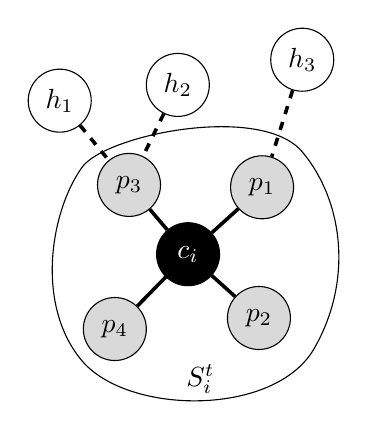
\begin{tikzpicture}[auto,vertex/.append style={minimum width=8mm}]
    \node[vertex,rare] (center) at (0,0) {$c_i$};
    \node[vertex,medium] (p1) at (.94,.85) {$p_1$};
    \node[vertex,medium] (p2) at (0.9,-.81) {$p_2$};
    \node[vertex,medium] (p3) at (-.75,.88) {$p_3$};
    \node[vertex,medium] (p4) at (-.93,-.95) {$p_4$};
    \node[vertex] (h1) at (-1.63,1.95) {$h_1$};
    \node[vertex] (h2) at (-0.13,2.15) {$h_2$};
    \node[vertex] (h3) at (1.45,2.47) {$h_3$};
    \foreach \source/\dest in {center/p1,center/p2,center/p3,center/p4}
    \draw[edge] (\source) edge  (\dest);
    \foreach \source/\dest in {h3/p1,h2/p3,h1/p3}
    \draw[edge, dashed] (\source) edge  (\dest);

    \draw[] (1.45, 1.3) 
    .. controls ++(130:.81) and ++(55: .51) .. (-1.35, 1.1)
    .. controls  ++(55: -.71) and ++(130:.91) .. (-1.35,-1.35)
    .. controls  ++(130: -.91) and ++(240:1) .. (1.6,-1.2) node[pos=.5,above=-1pt] {$S_i^t$}
    .. controls  ++(240: -1) and ++(130:-.81) .. cycle ;
  \end{tikzpicture}
\end{document}
